\documentclass[11pt,letterpaper,notitlepage]{article}

% Codificación GNU/Linux
\usepackage[utf8]{inputenc}
\usepackage[activeacute,spanish]{babel}

% Margenes
\usepackage{anysize}
\marginsize{2cm}{2cm}{2cm}{2cm}

% Simbolos y letras para matemáticas
\usepackage{amssymb,amsmath,amsfonts}

% Colores
\usepackage{color}
\definecolor{rojo}{RGB}{255,26,34}
\definecolor{gris}{RGB}{104,108,113}

% Elementos Flotantes (Figuras y Tablas)
\usepackage{graphicx}
\graphicspath{ {img/} }
\usepackage{float}
\usepackage{multicol}
\usepackage{multirow}
\usepackage{subfigure}
\usepackage{epstopdf}
\usepackage{enumerate}
\usepackage{hyperref}
\hypersetup{
    colorlinks,
    linkcolor={gris},
    citecolor={gris},
    urlcolor={gris}
}
\usepackage{color}
\definecolor{gray}{rgb}{0.8,0.8,0.8}
\usepackage{listings}
\lstset{ %
  backgroundcolor=\color{gray},  % keyword style
  language=c++                 % the language of the code
}
\usepackage{siunitx}

\begin{document}

% Cabezera
\begin{figure}
\vspace*{-1cm}
\begin{minipage}[c]{0.4\textwidth}
	
\includegraphics[width=0.5\textwidth]{fcfm}
\end{minipage}
\hfill
    \begin{minipage}[t]{0.6\textwidth}
    %--------- Datos del curso ------------------
    \begin{flushright}
    	Laboratorio de Automática\\
    	Otoño 2016 \\
    \end{flushright}
\end{minipage}
\rule{\linewidth}{.4mm}
\end{figure}

%--------- Datos del documento -------------
\begin{center}
\Large \textbf{Control de velocidad de motor de corriente continua} \\
\large \textbf{Tema: Sintonización de controladores PI}\\
\large Profesor: Roberto Cárdenas\\
\large Profesor Auxiliar: Romina Arriaza\\
\large Ayudantes: Cristián Retamal, Pablo Fuentes, Rodrigo Muñoz\\
\end{center}

\section{Introducción}

En esta experiencia de laboratorio tiene como objetivo diseñar e implementar un controlador PI digital para el control de velocidad de un motor de corriente continua. La sintonización del controlador se realizará usando el método de Ziegler-Nichols (Z\&N).

\subsection{Descripción de la planta}

Una de las principales ventajas del motor de corriente continua (C.C.) corresponde la facilidad con que puede controlarse su velocidad, la posibilidad de alcanzar grandes velocidades y los elevados torques de arranque. Así, aún cuando los motores de C.C. están siendo reemplazados cada vez más por motores de inducción trifásicos con control electrónico de velocidad, todavía se les encuentra en algunos procesos industriales y, sobre todo, en tracción eléctrica (Metro, ferrocarriles, tranvías, etc.).

El motor C.C. del laboratorio de automática se encuentra conectado en una configuración de excitación independiente, de esta forma el circuito de campo esta alimentado de forma independiente por una fuente de poder de $50 \,\mbox{\si{\volt}}$. Un PLC (\textit{programmable logic controller}) esta conectado al motor de tal forma que puede modificar el voltaje de armadura ($0 \, \mbox{\si{V}} \leq V_a \leq 10 \, \mbox{\si{V}}$) y obtener una medición de velocidad a través de un encoder incremental conectado al eje del rotor. El sistema de control se presenta al usuario a través de una plantilla Simulink, como se muestra en la Figura \ref{esquema-planta}.

\begin{figure}[H]
\begin{center}
	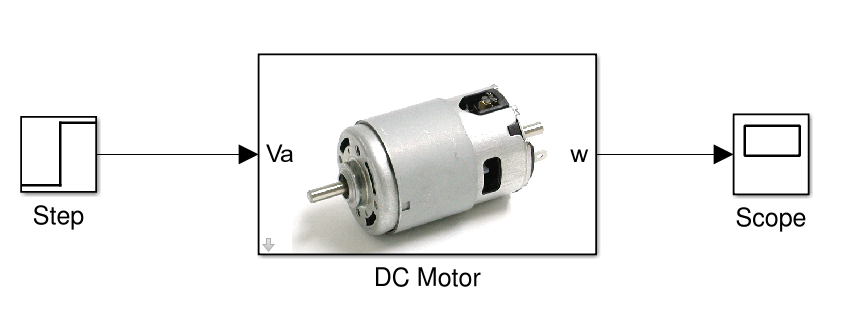
\includegraphics[width=0.5\textwidth]{planta}
	\caption{Plantilla Simulink para el control del motor C.C.}
	\label{esquema-planta}
\end{center}
\end{figure}


\section{Sintonización de un control PI mediante simulación}

Mediante pruebas de laboratorio sobre el motor, se obtiene una función de transferencia \ref{tf} de la planta que relaciona la velocidad de giro del motor con el voltaje de armadura ($0 \, \mbox{\si{V}} \leq V_a \leq 10 \, \mbox{\si{V}}$), utilizando un tiempo de muestreo de $T_s = 0.05 \,\mbox{\si{s}}$.

\begin{equation}
\label{tf}
G(z) = \frac{4.191 \cdot 10^{-5} z^{-1}}{  1 - 1.989 z^{-1} + 0.9895 z^{-2}}
\end{equation}

Para el diseño de los controladores discretos, se solicita que el sistema retroalimentado siga la siguiente referencia de velocidad:

\begin{equation}
\label{ref-r}
r(t) =
  \begin{cases}
    1.5 & \quad 0 \,\mbox{\si{\second}} \leq t < 50 \,\mbox{\si{\second}}\\
    2.5 & \quad 50 \,\mbox{\si{\second}} \leq t < 100 \,\mbox{\si{\second}}\\
  \end{cases}
\end{equation}



\section{Actividades de simulación}

\begin{enumerate}[\bfseries {A}1]

\item Dibuje un esquema de diagrama de bloques en lazo cerrado del sistema, indicando claramente tanto la variable manipulada como la variable controlada. Además, especifique el sensor utilizado, un actuador y posibles perturbaciones relevantes a la planta.

\item Describa el método de Z\&N para construir un controlador PI empleando la curva de reacción del sistema. ¿Cuáles son las diferencias entre la técnica LGR y el método de Z\&N?

\item Diseñe un controlador PI mediante simulación utilizando el método de curva de reacción de Z\&N. Recuerde que para obtener los parámetros debe realizar la prueba en lazo abierto.

\item Simule los resultados del controlador y estime su desempeño utilizando como métricas el sobrepaso y tiempo de establecimiento.

\end{enumerate}


\section{Actividades usando la planta real}

\begin{enumerate}[\bfseries {B}1]

\item Implemente el controlador obtenido en sección anterior y compare los resultados conseguidos con la simulación previamente realizada.

\item Realice la prueba de lazo de abierto en la planta y obtenga los parámetros de un control PI mediante Z\&N, compárelos con los obtenidos mediante la simulación e implémentelo en el sistema con la referencia $r(t)$ propuesta anteriormente. Analice el comportamiento del motor, mostrando variable controlada y manipulada.

\item Mencione ventajas y desventajas de utilizar el método de Z\&N.


\end{enumerate}



\end{document}